
\runningheader{Oppgave p)}{}{Side \thepage\ av \numpages}


% ********************************************************
% oppgave p) 
% ********************************************************  
  \item[p)]
    I denne oppgaven skal du integrerer
    følgende 3 signal.
\begin{align}
  \label{eq:213}
  u_{1}(t) & = 0.5 \sin(0.3 t) \\
  \label{eq:211}
  u_{2}(t) & = 0.5 \sin(0.55 t)\\
  \label{eq:211s}
  u_{3}(t) & = 0.5 \sin(0.8 t)
\end{align}
Hensikten med oppgaven er å vise hvordan disse 3 sinussignalene henger  
sammen med {\sf Chirp}-blokken. 
Kjør først filen \fbox{\tt oving2\_data.m}, og lag deretter
   modellen vist under
      \begin{figure}[H]
    \centering
    \hspace*{0mm}\scalebox{0.8}{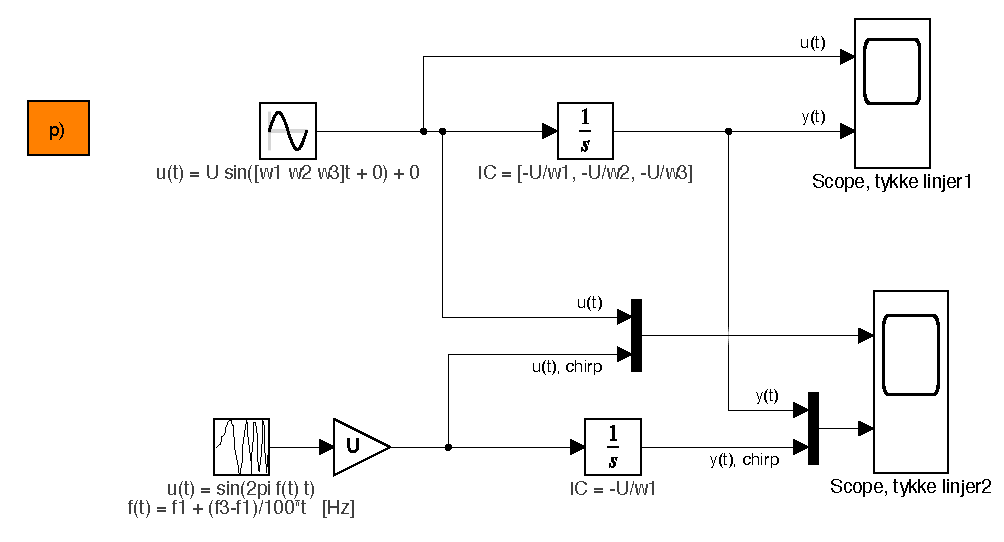
\includegraphics{2p.pdf}}
  \end{figure}
  {\color{red}La simuleringstiden nå være 100 sekund.  }
  
  \begin{itemize}
  \item   I  {\sf  Sine Wave}-blokken
 spesifiserer du {\tt Frequency}-feltet som {\sf [w1, w2, w3]}. 
\item   I  {\sf  Chirp}-blokken
  spesifiserer du
  \begin{itemize}
  \item 
  {\sf f1} som {\tt Initial frequency},
  \item 
  {\sf f3} som {\tt Target frequency} og
  \item 
  {\sf 100} som {\tt  Target time} (tilsvarer simuleringstiden).
  \end{itemize}
  \item Spesifiser initialverdiene som
    vist i figuren slik at cosinuskurvene svinger omkring $y{=}0$.
  \end{itemize}

    {\bf Gjør følgende oppgaver / svar på følgende spørsmål:    }
    
  \begin{enumerate}[label=p\arabic*)]
    \item Simuler modellen og vis at du får et resultat som ligner på 
responsen i figur~\ref{fig:dump_2p}, hvor 
vi har endret den svarte kurven til stiplet slik at
det er lettere å identifisere {\sf Chirp}-signalet.

Ta med simuleringsresulatet
i innleveringen din
ved å bruke prosedyren på
     side~\pageref{page:prosedyre}.

  \begin{figure}[H]
    \centering
    \hspace*{0mm}\scalebox{0.55}{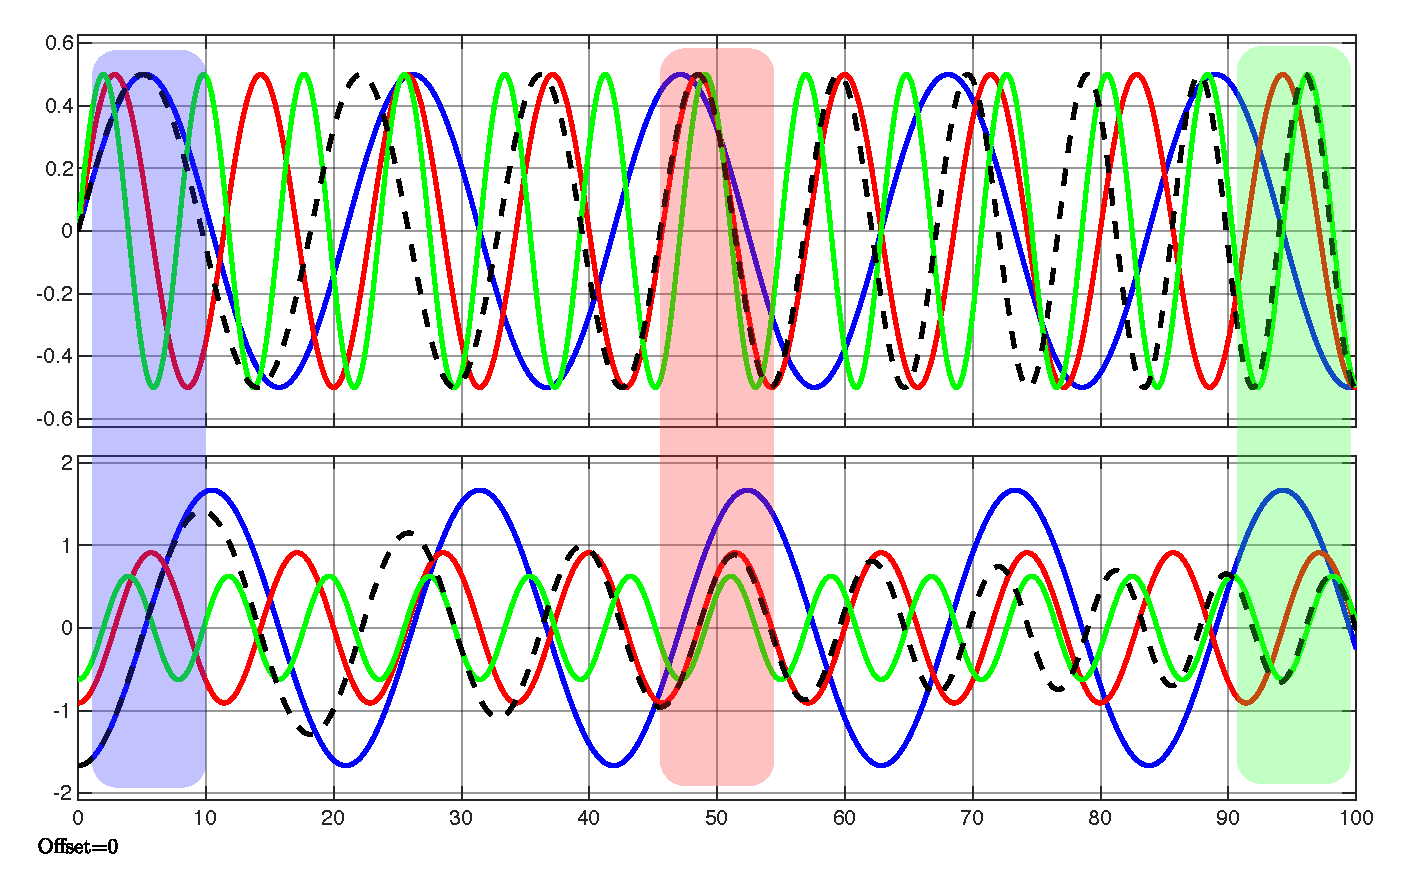
\includegraphics{fig_2p.pdf}}
    \caption{Simuleringsresultat. De fargelagte områdene er gjort i
      tegneprogram etterpå. }
    \label{fig:dump_2p}
  \end{figure}

 Som du ser
``overlapper'' det svart-stiplede chirp-signalet
\begin{itemize}
\item med den blå sinuskurven i det blå feltet i begynnelsen,  
\item med den røde sinuskurven i det røde feltet i midten,  
\item med den grønne sinuslurven i det grønne feltet kurven i slutten  
\end{itemize}
og dette gjelder både i den øverste og nederste delfiguren.


\item Som du ser så reduseres amplituden $Y$ i integralet $y(t)$ når
  frekvensen $\omega$ øker.   
  Forklar, ut fra et matematisk ståsted, hvorfor dette skjer? I
  forklaringen din kan du ta
  utgangspunkt i at uttrykket for $y(t)$ er gitt av
  følgende sammenheng.
\begin{align}
  y(t) & = \int_{0}^{t} u(\tau)  d\tau + y(0)  \notag \\
       & = \int_{0}^{t} U{\cdot}\sin(\omega{\cdot}\tau) d\tau  +y(0) \notag   \\
  & = \ldots \notag   \\
  & = \ldots \notag   
\end{align}

Fortsett på denne utledningen og finn det analytiske uttrykket for
$y(t)$, og bruk dette til å forklare hvorfor amplituden til $y(t)$ synker med
økende frekvens~$\omega$. 
  
\end{enumerate}




 
